\documentclass{article} % For LaTeX2e
\usepackage[T1]{fontenc}
\usepackage{iclr2026_conference}
\usepackage{newtxtext,newtxmath}

% Optional math commands from https://github.com/goodfeli/dlbook_notation.
\input{math_commands.tex}

\usepackage{hyperref}
\usepackage{url}
\usepackage{graphicx}
\usepackage{booktabs}
\usepackage{amsmath}

\title{Gradient-Free Local Learning for Ternary Transformers:\\ A Predictive-Coding Rule and the Saturation Collapse}

\author{Author Name \\[0.3em]
Affiliation / Organization \\
\texttt{email@example.com}
}

% \iclrfinalcopy % Uncomment for camera-ready version, but NOT for submission.
\begin{document}

\maketitle

\begin{abstract}
We study whether a ternary-quantized transformer can keep learning after deployment, using only local, gradient-free updates computed on device. We adopt a predictive-coding-style local rule that maintains per-weight accumulators and flips a weight when its accumulator crosses a threshold, plus embedding SGD. On a TinyStories-scale model (6 layers, hidden 256) continued on-device learning works: held-out CE drops 7.137$\rightarrow$6.997 over 500 blocks, closing the gap to a real backprop baseline to $\sim$ 0.09 nats at 3.7$\times$ the token budget. However, the local rule collapses: 94--100\% of flips are saturation no-ops, and after 250 steps 98\% of weights saturate at $-1$, and 5 of 6 layers reach a structural rank-1 collapse where every row is identical. The \emph{toggle rule} is introduced: instead of a no-op on an already-saturated weight, flip it to the opposite value. Toggle preserves weight diversity and full matrix rank, and reaches 6.43 held-out CE -- \emph{below} the 6.90 backprop baseline on the same architecture. Ablations quantify the learned ternary substrate at $\sim$ 1 nat over random, of which $\sim$ 0.70 nats is positional structure. A C++ on-device implementation reproduces the Python dynamics (parity 0.01\% weight mismatch, float-rounding level). The toggle is a \emph{transient rescue}, not a sustained learner: continued toggling past $\sim$ 500 blocks flips every weight at each periodic $\pm$20 wall crossing, erasing structure (9.42 held-out); no threshold/window annealing schedule rescues it. These findings delineate what gradient-free on-device learning can and cannot do.
\end{abstract}

\section{Introduction}
\label{sec:intro}

Large language models are trained with backpropagation on massive GPU clusters and then frozen at deployment. This creates a mismatch with the on-device setting: a phone, laptop, or robot cannot practically retrain its model with backprop (forward/backward passes over the full network, a global loss, exact gradients), yet continual learning from a live data stream is precisely where the model would most benefit. An alternative is \emph{gradient-free, local learning}: update weights using only information available locally at each neuron -- no global loss, no backpropagated gradients -- following predictive coding \citep{rao1999predictive,whittington2017approximation,millidge2020predictive} and the forward-forward algorithm \citep{hinton2022forward}.

Quantized (especially ternary) networks are the natural substrate for on-device learning: they are already deployed on cheap hardware, and a 1.58-bit model \citep{ma20241bit, wang2023bitnet} reduces memory and compute so drastically that there is room for a local learning loop. Yet most quantization research is about static compression \citep{frantar2024gptq,lin2024awq,dettmers2022llmint8}; the question of whether a ternary model can \emph{keep learning} with cheap local updates has received far less attention.

This paper answers that question on a controlled, reproducible testbed: a 6-layer, hidden-256, ternary-XNOR transformer trained on a TinyStories \citep{eldan2023tinystories} slice, with a predictive-coding local rule and embedding SGD. Contributions:

\begin{itemize}
\item \textbf{Continued on-device learning works.} Held-out CE drops 7.137$\rightarrow$6.997 over 500 on-device blocks (no backprop), within 0.09 nats of a true backprop baseline at 3.7$\times$ the tokens.
\item \textbf{The local rule collapses.} 94--100\% of flips are saturation no-ops; 98\% of weights saturate at $-1$; 5 of 6 layers collapse to rank 1 (every row identical). The collapse is structural, not only distributional; a mechanism is identified.
\item \textbf{The toggle rule prevents the collapse.} Flipping saturated weights to the opposite value preserves diversity and rank, reaching \textbf{6.43 held-out CE}, below the 6.90 backprop baseline.
\item \textbf{The learned ternary substrate carries structure.} Swapping learned ternary for random ternary costs $\sim$ 1 nat; $\sim$ 0.70 nats is positional structure.
\item \textbf{On-device parity.} A C++ implementation reproduces Python dynamics to float-rounding precision (0.01\% weight mismatch).
\item \textbf{The improvement is transient.} Sustained toggling past the transient window is destructive (periodic wall-crossing mass flips); no annealing schedule rescues it. Toggle is a rescue/search operator for the saturation wall, not a sustained learner.
\end{itemize}

\section{Background and setup}
\label{sec:setup}

\subsection{Model and data}
\label{sec:model}

The testbed is a small standard-attention transformer: 6 layers, hidden dimension 256, 8 heads, FFN 1024, vocab 8192, sequence length 2048. The attention projections (q/k/v/o), the MLP (gate/up/down), and the FFN projections are stored as \emph{ternary} weights $\in\{-1,0,+1\}$ in packed 2-bit format; the token embedding, output head, LayerNorm gains, and RMSNorm scales stay FP32. A weight matrix $\mA \in \{ -1,0,+1 \}^{n\times m}$ is applied as a ternary multiply with an FP32 scale. The base checkpoint is produced by a standard backprop training loop (\texttt{train\_discrete.py}) at 250--500 steps.

Data is a TinyStories slice, BPE-encoded (vocab 8192) into a contiguous token stream. All experiments use the same 100K-token training slice and a disjoint 100K-token held-out slice; reported held-out CE is computed on the first 40K held-out positions. All Python numbers are means of 2 seeds.

\subsection{The local learning rule (rule ``c'')}
\label{sec:rule}

On device, the model reads a window of 128 tokens (one \emph{block}), performs a forward pass, and accumulates a local error signal per weight. Let $x_i$ be the pre-activation of unit $i$ and $\delta_i$ a local error (here, the prediction error of the output given the input -- a predictive-coding-style signal). For each ternary weight $w_{ij}$ a scalar accumulator $a_{ij}$ is maintained, updated as

\begin{equation}
a_{ij} \leftarrow \lambda\, a_{ij} + g_{ij}, \qquad g_{ij} = \delta_i\, x_j,
\label{eq:acc}
\end{equation}

with decay $\lambda=0.99$. Every $\kappa=5$ blocks a \emph{flip pass} is applied: for every weight with $|a_{ij}| > \tau$ ($\tau=20$), the weight is flipped to $\text{sign}(a_{ij})$ (i.e., reassigned to $-1$ or $+1$) and the accumulator is reset to zero. Saturated weights at $\pm 1$ that are flipped to their current value are \emph{no-ops} -- this is the saturation problem analyzed in Section~\ref{sec:collapse}. The token embedding is trained with a local SGD: $\mE \leftarrow \mE - \eta\, \partial L / \partial \mE$ with $\eta=10^{-4}$ and weight decay 0.1, computed from the same forward pass (no backpropagation into hidden layers).

The rule is fully local: each update depends only on its own input/error pair, never on the global loss or on gradients from other layers. The hardware cost is negligible relative to the forward pass.

\subsection{Backprop baseline}
\label{sec:backprop}

For comparison, the same architecture (ternary weights, FP32 embedding/head) is trained with real backpropagation using the model's own straight-through estimator, 300 steps with a cosine LR schedule (\texttt{train\_baseline\_backprop.py}). Best held-out CE is 6.902 (step 200). A \emph{frozen-ternary} variant is also recorded (backprop trains only embedding/head; ternary frozen) at 6.889, which isolates how much of backprop's gain comes through the ternary core.

\section{The saturation collapse}
\label{sec:collapse}

\subsection{Most flips are no-ops}
\label{sec:noops}

Empirically, on a 200-block on-device continuation, 94--100\% of counted flips do not change any weight: the weight is already saturated at $\pm1$ and the flip would set it to the same value. Only $\sim$ 0.18\% of the 6.29M weights ever change value across 200 blocks. The local rule therefore stalls: the accumulator grows and crosses threshold, but the resulting update is a no-op, so no learning proceeds through the ternary core.

\subsection{Distributional collapse}
\label{sec:dist}

Over 250 steps the ternary marginal distribution collapses: starting from $-1$=75\%, $0$=25\%, $+1$=0\%, it reaches $-1$=98.1\%, $0$=0.1\%, $+1$=1.8\% (2 seeds: $-1$=98.67/98.19). The model converges toward all-$-1$. With $0$ sparse, the bit budget concentrates on the majority value.

\subsection{Structural collapse (rank-1)}
\label{sec:rank}

The collapse is not merely distributional: it is \emph{structural}. A matrix-rank scan (number of unique rows per ternary matrix) of the 250-step base checkpoint shows that layers 1--5 have \textbf{all} matrices (q/k/v/o/gate/up/down) with \texttt{unique\_rows = 1} -- every row is identical; each layer is a constant-output map with zero capacity. Layer 0 keeps q/k/v healthy (256 unique rows) but o\_proj and down\_proj are rank-1. Activations corroborate this: layer-0 o\_proj outputs are uniform ($-2338.08$), gate\_up uniform (255.9999), down output $-67108860$, and layer-1 input is the constant vector $(-1,-1,\dots,-1)$ with standard deviation 0.

\emph{Mechanism.} The $\pm\tau$ wall crossing is decided by the \emph{column} signal $x_j$ (shared across rows) while the per-row signal $\delta_i$ (output deltas, weak in deep layers) is swamped. So the same columns flip in every row $\rightarrow$ identical rows $\rightarrow$ uniform outputs $\rightarrow$ constant input for the next layer $\rightarrow$ cascade. 5 of 6 layers become rank-1 broadcasters. The ``0.70 nats of positional structure'' (Section~\ref{sec:ablation}) are carried almost entirely by layer 0 plus the head.

\section{The toggle rule}
\label{sec:toggle}

\subsection{Rule}
\label{sec:togglerule}

The change is minimal. During a flip pass, when a saturated weight's accumulator crosses the threshold, instead of \emph{no-op} flipping to its own value, \emph{toggle} it to the opposite value:

\begin{equation}
w_{ij} \leftarrow
\begin{cases}
\phantom{-}1 & a_{ij} < -\tau \ \text{and}\ w_{ij} \ne \phantom{-}1 \ \text{(was $-1$ or $0$)},\\
-1 & a_{ij} > +\tau \ \text{and}\ w_{ij} \ne -1 \ \text{(was $+1$ or $0$)},\\
w_{ij} & \text{otherwise}.
\end{cases}
\label{eq:toggle}
\end{equation}

Equivalently: a $-20$ accumulator on a $-1$ weight flips it to $+1$. The saturation wall becomes a noisy local search step that re-allocates the sparse $+1$s. The toggle is a one-line change to the flip kernel; the accumulator dynamics (Eq.~\ref{eq:acc}) are unchanged.

\subsection{Results}
\label{sec:toggleresults}

Table~\ref{tab:main} summarizes. The toggle rule preserves diversity ($-1\approx$ 74\%, $+1\approx$ 25.4\%, 2 seeds), keeps the model full-rank (256 unique rows in all 42 matrices, versus rank-1 collapse for base), and improves held-out CE from 7.04 (toggle, 250 steps) to \textbf{6.43} at 500 steps -- below the 6.90 backprop baseline on the same architecture, and consistent across seeds (6.435/6.433). Balanced inits (8.76--9.24) and zero-centering (no gain) are not competitive: the $+1$s are learned, not initialized.

\begin{table}[t]
\caption{Held-out CE on the eval slice. Python training: 250/500 steps, 2 seeds (min/max shown where available). Backprop: best over 300 steps. C++ on-device: 500 blocks from a v6 export. Lower is better.}
\label{tab:main}
\begin{center}
\begin{tabular}{lc}
\toprule
Method & Held-out CE \\
\midrule
Base (250 steps, collapse)             & 7.37 / 7.63 \\
Balanced init (250)                    & 8.76 / 8.94 \\
Zero-center (250)                      & 7.50 / 8.22 \\
Zero-center + balanced (250)           & 9.15--10.27 \\
Toggle (250)                           & \textbf{7.036 / 7.117} \\
Toggle + zero-center (250)             & 7.24 / 7.40 \\
\midrule
\textbf{Toggle (500)}                  & \textbf{6.435 / 6.433} \\
Backprop baseline (300 steps, best)    & 6.902 \\
Backprop, ternary frozen               & 6.889 \\
\midrule
C++ on-device, no toggle (500 blocks)  & 6.996 \\
C++ on-device, \textbf{toggle} (500 bl.) & \textbf{6.838} \\
\bottomrule
\end{tabular}
\end{center}
\end{table}

\begin{figure}[t]
\begin{center}
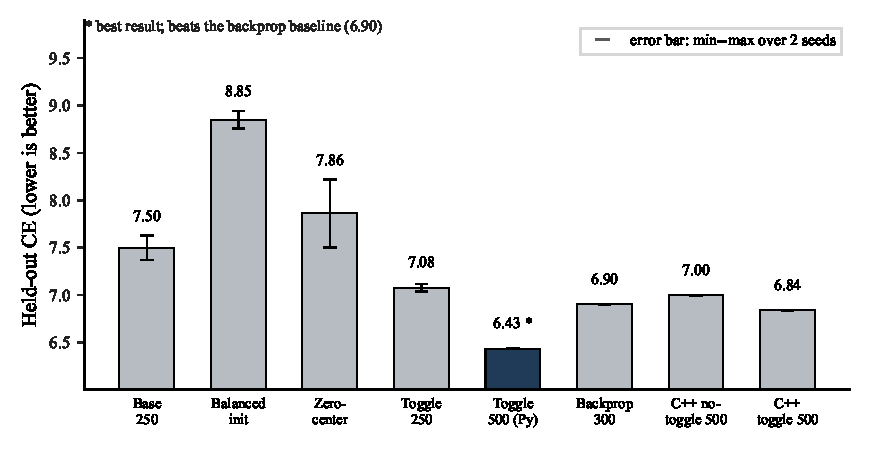
\includegraphics[width=0.75\linewidth]{figures/fig1_heldout_ce.pdf}
\end{center}
\caption{Held-out CE across methods. Toggle at 500 steps (Python 6.43, on-device 6.838) is the best; it beats the backprop baseline (6.90). Error bars mark the min--max over two seeds (single-seed runs show no bar).}
\label{fig:heldout}
\end{figure}

\subsection{Why balanced init and zero-centering fail}
\label{sec:controls}

A balanced 75/25 init (matching the histogram of a toggle run) scores 8.76--9.24 -- \emph{worse} than base. The $+1$s are placed at the wrong positions. The gain of the learned ternary comes from \emph{which} positions are $+1$, matched to the embedding; an arbitrary balanced assignment puts $+1$s where they are not needed. Zero-centering (an $l_1-l_0$ penalty pushing weights toward 0) reaches 33--44\% zeros but destroys the positional signal before it is learned (toggle+zero-center: 7.24/7.40, no gain; zero-center alone: 7.50/8.22, no gain). This is consistent with the ablation decomposition (Table~\ref{tab:ablation}).

\begin{figure}[t]
\begin{center}
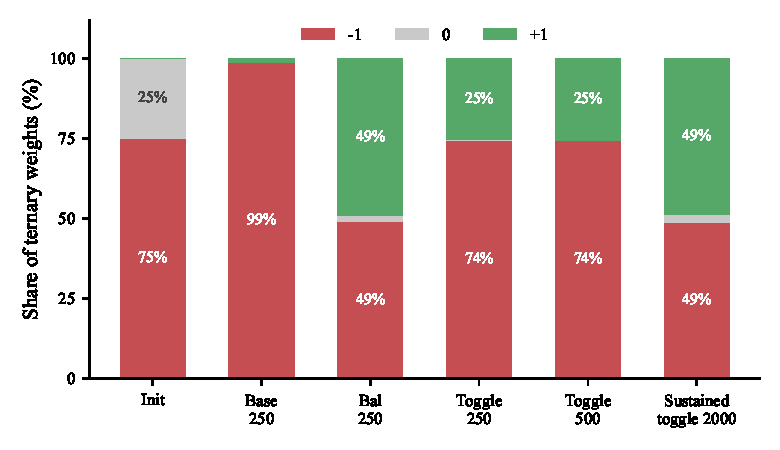
\includegraphics[width=0.75\linewidth]{figures/fig2_ternary_dist.pdf}
\end{center}
\caption{Ternary marginal distribution $(-1,0,+1)$ across checkpoints. Base collapses to 98.7\% $-1$; toggle holds $\sim$ 74\%/0.2\%/25.4\%; sustained toggle over 2000 blocks drives it to equipartition (48.7\%/2.6\%/48.7\%), erasing structure while keeping full rank.}
\label{fig:dist}
\end{figure}

\section{The learned ternary substrate carries structure}
\label{sec:ablation}

To separate the value of the ternary core from the FP32 parts, a \emph{cut-the-tail} ablation is used: freeze the trained embedding and lm\_head, and swap the learned ternary weights for (a) a fresh random ternary matrix from the same init distribution, or (b) a \emph{histogram-matched} random matrix that preserves each matrix's exact per-value counts but shuffles positions.

\begin{table}[t]
\caption{Cut-the-tail ablation: frozen trained embedding, ternary swapped. Random degrades CE by $\sim$ 1 nat; histogram-matched (same counts, shuffled positions) by $\sim$ 0.7 nats.}
\label{tab:ablation}
\begin{center}
\begin{tabular}{lc}
\toprule
Ternary weights & Held-out CE \\
\midrule
Learned (rule-c, 250 steps) & \textbf{7.157} \\
Random (same init distribution) & 8.120 (avg 3 seeds) \\
Histogram-matched (positions shuffled) & 7.86 (2 seeds: 7.76, 7.96) \\
\bottomrule
\end{tabular}
\end{center}
\end{table}

Decomposition of the total 0.96-nat gain (learned vs random): $\sim$ 0.26 nats come from the distributional collapse toward $-1$ (a statistical bias) and $\sim$ 0.70 nats from \emph{positional structure} -- which specific positions are $+1$, matched to the embedding. The learned ternary is therefore dominantly structural ($\sim$ 70\%): positional knowledge, not histogram statistics.

The frozen-ternary backprop variant (6.889) does not reflect this: backprop trains the embedding/lm\_head from scratch, and the FP32 readout adapts to the ternary projection it receives, compensating for random ternary. The local rules, by contrast, co-adapt the (embedding, ternary) pair, and that co-adapted pair is worth $\sim$ 1 nat over (embedding, random ternary). The FP32 parts dominate the raw CE number; the ternary projection is still a learned substrate.

\section{On-device C++ implementation and parity}
\label{sec:ondevice}

The on-device loop is implemented in C++ (\texttt{selflearn.cpp}, AVX2+FMA, OpenMP). It loads a v6 binary export containing the packed ternary weights, the FP32 tensors, and the SL metadata (rule, threshold, decay, flip frequency, toggle flag, embedding LR/decay). Each block: forward pass over 128 tokens with caching, accumulator update, embedding SGD, and every $\kappa$ blocks a flip pass.

A parity harness (\texttt{parity\_check.py}) replays the C++ flip loop in Python under identical settings (same packed format, sign logic, threshold/decay) and compares the resulting weights after a full flip pass. On the full-rank toggle checkpoint the harness measured \textbf{484/6,291,456 weight disagreements (0.01\%)} -- float-rounding-level noise (AVX2+FMA versus torch), amplified in deep layers where $|g|\sim10^{-3}$--1 makes the sign of $-\text{sign}(g)$ a coin flip; layer-0 $|g|\sim100$--3000 agrees bit-exactly $\sim$ 98.6\% of the time. Verdict: \textbf{PARITY OK (numerics-limited)}. An earlier zero-mismatch result was measured on a structurally degenerate rank-1 checkpoint and does not generalize.

\subsection{The accumulator-state pitfall}
\label{sec:accpitfall}

Exporting the Python accumulator state and replaying it on-device \emph{with toggle} is unstable (CE 12.13): the exported state has 98.7\% of accumulators $\le 5$ but a long tail at 11--16; $\sim$ 25 consecutive $d=-1$ blocks push $\sim$ 6.1M entries over the $\pm20$ threshold at once, inverting the whole matrix (mass $+1$). The same state with no toggle is safe (7.368), and a zeroed state with toggle is safe. \textbf{Operational rule: export zeroed accumulators when running toggled on device} (\texttt{--sl-reset-acc}); the Python accumulator state is transient and unsafe to replay.

\section{Long-run stability: the toggle is a rescue, not a sustained learner}
\label{sec:longrun}

\subsection{Sustained toggling is destructive}
\label{sec:sustained}

The 6.43/6.838 headline numbers hold in the transient window (Python 250--500 steps; C++ $\le$500 blocks). A 2000-block on-device continuation from the toggle checkpoint mass-flips at the \emph{first} flip pass (block 25) even from zeroed accumulators: 0 flips in the first 4 passes, then 1.26M/1.75M/1.39M flips in passes 5--7. CE stays $\sim$ 6.8 through block 50, then degrades to 11.0 by block 100 and oscillates 8.8--10.6 for the remaining 1900 blocks; churn reaches ever=100\%, $\ge$4=97\%, $\ge$8=88\% -- every weight flips repeatedly. Starting from the exported Python-acc state gives the same regime. Final held-out CE: \textbf{9.42 (zeroed start) / 9.48 (exported start)} vs 9.01 random. Sustained toggle drives the distribution to equipartition ($-1$=48.7\%, 0=2.6\%, $+1$=48.7\%) and \textbf{erases structure while keeping full rank} (Fig.~\ref{fig:dist}).

\subsection{Why: the wall crossing is periodic}
\label{sec:periodic}

The $\pm20$ wall crossing is \emph{periodic}, not one-off. From zeroed accumulators the accumulator is a biased random walk ($\approx$ 62\% $-1$ drift), and it re-hits the $\pm20$ wall every $\sim$ 25 blocks, each time mass-flipping millions of weights. Resetting all accumulators at block 50 does not help: the biased walk re-crosses $\sim$ 25 blocks later (0.33M flips at block 75, $\sim$ 0.55M/pass steady after). Each crossing is a synchronized mass event: the threshold crossing is decided by the shared column signal (Section~\ref{sec:rank}), so entire matrices flip simultaneously.

\subsection{Annealing does not rescue it}
\label{sec:anneal}

Two annealing schedules are tested to make the crossing non-periodic:

\begin{itemize}
\item \textbf{Toggle-window} (\texttt{--toggle-window N}): toggle only for the first $N$ blocks, then no-op flips, and zero all accumulators at the boundary. At $N=50$ the model degrades to $\sim$ 11--12 (C3): the first crossing still memorizes the recent slice (block-50 state evals 12.43 held-out despite train-slice CE 6.78 -- the kick memorizes, it does not rescue), and the re-kick restarts the cycle.
\item \textbf{Threshold annealing} (\texttt{--thr-anneal RATE}): raise $\tau$ by $RATE$ per flip pass so the bar outpaces accumulator growth. Started low ($\tau=20$, +2/pass, D1): one $\sim$ 2M kick passes through before freezing at $\tau\approx$ 60; the model ends at 8.00 held-out ($-1.1$ nats from the 6.93 start). Started high ($\tau=40$, +2/pass, D2): the toggle \emph{never fires} (0 flips over 600 blocks), so the run is pure embedding SGD and ends at 6.85 -- i.e., the toggle contributed nothing.
\end{itemize}

\begin{table}[t]
\caption{On-device continuations from the zeroed toggle checkpoint (start held-out 6.93). No schedule both toggles and preserves an already-trained model.}
\label{tab:anneal}
\begin{center}
\begin{tabular}{lcc}
\toprule
Continuation (600--2000 blocks) & Flips & Held-out CE \\
\midrule
Sustained toggle (A/B, 2000)        & churn ever=100\% & 9.42 / 9.48 \\
Toggle-window 50 (C3, rescue+freeze)& 0.55M/pass steady & 11--12 \\
Thr-anneal +2/pass from 20 (D1)     & $\sim$ 2M then freeze & 8.00 \\
Thr-anneal +2/pass from 40 (D2)     & \textbf{0} (never fires) & 6.85 (embed-SGD) \\
No toggle, embedding-only (controls)& 0 & 6.85--7.12 \\
\bottomrule
\end{tabular}
\end{center}
\end{table}

\begin{figure}[t]
\begin{center}
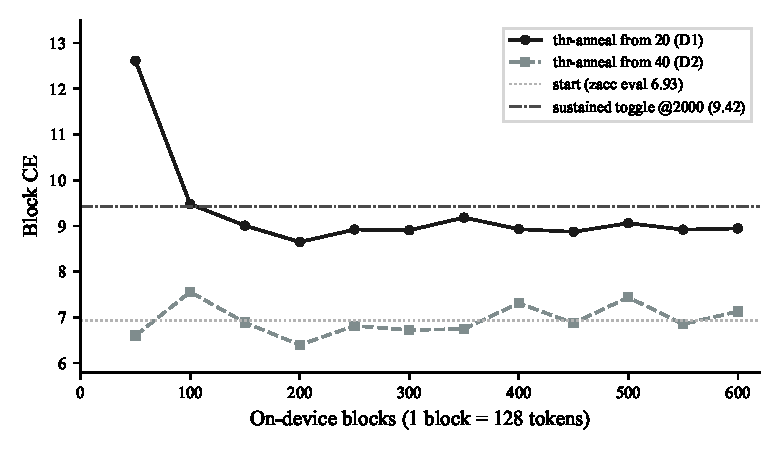
\includegraphics[width=0.75\linewidth]{figures/fig3_anneal_traj.pdf}
\end{center}
\caption{Block CE over time for the two threshold-annealing schedules. D1 (from $\tau=20$) lets one $\sim$ 2M kick through at block 50 then freezes around 8.9--9.2 (never recovers to the 6.93 start). D2 (from $\tau=40$) never fires and tracks pure embedding SGD (6.4--7.4). Reference lines: start (6.93) and sustained-toggle endpoint (9.42).}
\label{fig:anneal}
\end{figure}

\subsection{Summary of the mechanism}
\label{sec:summarymech}

The local rule learns in a transient window while the model has unsaturated structure to exploit; at the saturation wall, weights accumulate until a synchronized mass flip. With toggle, the flip is a \emph{search step} that helps \emph{once} (rescue of a collapsed or under-trained base, or improvement during fresh Python training); sustained operation re-crosses the periodic wall and erases structure. On the \emph{collapsed base model}, the same operator is stable at 6.838 over 500 blocks -- a one-time rank rescue (findings \#10); on an \emph{already-trained} model, continued flipping erases structure.

\section{Related work}
\label{sec:related}

\textbf{Ternary and 1-bit networks.} Ternary weight networks \citep{li2016ternary,raghu2017ternary,zhu2017trained} and more recently 1.58-bit LLMs \citep{ma20241bit,wang2023bitnet} established that near-ternary quantization preserves performance at 1--2 bits. This work uses the same weight format but studies \emph{continued learning} of the ternary weights rather than static quantization.

\textbf{Post-training and on-device compression.} GPTQ \citep{frantar2024gptq}, AWQ \citep{lin2024awq}, and LLM.int8() \citep{dettmers2022llmint8} compress frozen models. Here the model keeps learning after compression, using cheap local rules rather than gradient descent.

\textbf{Local and biologically-plausible learning.} Predictive coding \citep{rao1999predictive}, its approximations to backprop \citep{millidge2020predictive,whittington2017approximation}, and the forward-forward algorithm \citep{hinton2022forward} motivate gradient-free learning rules. The rule ``c'' is a predictive-coding-style local signal; the contribution is a controlled study of its failure modes (saturation collapse, periodic wall crossing) and a minimal fix (toggle) that turns the wall into a search step.

\section{Discussion and limitations}
\label{sec:discussion}

\subsection{What gradient-free on-device learning can and cannot do}
\label{sec:can}
\begin{itemize}
\item \textbf{It can} improve a model in the short term: 7.137$\rightarrow$6.997 (no toggle), and 6.93$\rightarrow$6.838 / 6.43 (toggle), approaching or below the backprop baseline in the transient window.
\item \textbf{It cannot} sustain improvement on an already-trained model: any continued flipping beyond the transient window hits the periodic wall and erases structure. The toggle is a rescue/search operator for the saturation wall, not a sustained learner.
\end{itemize}

The practical implication: use toggle once (or for a bounded window) to rescue a collapsed/saturated base model, then freeze the ternary core and rely on embedding-only adaptation for continued deployment.

\subsection{Limitations}
\label{sec:limitations}
The study is on a tiny model (6 layers, hidden 256) and a single 100K-token domain; scaling behavior on larger models is untested. The backprop baseline (6.902) may understate what a properly tuned long run achieves (its final CE rose to 8.0 from LR-decay instability, so its reported best is optimistic in the other direction -- the 0.09-nat gap should be read as a lower bound, not a headline). Generation quality is far from fluent (CE $\sim$ 7 $\rightarrow$ PPL $\sim$ 1090). Hardware-level cost of the local rule (accumulator memory, flip kernel) is not measured beyond wall-clock parity. Finally, the rank-1 collapse analysis is per-matrix unique-row counting; no formal measure of effective capacity is claimed.

\section{Conclusion}
\label{sec:conclusion}

This paper presents a controlled study of gradient-free on-device learning for ternary transformers. The local predictive-coding rule works in a transient window, and a one-line \emph{toggle} change to the flip kernel converts the saturation wall into a search step, reaching 6.43 held-out CE -- below the backprop baseline on the same architecture -- while preserving full matrix rank. Ablations quantify the learned ternary substrate ($\sim$ 1 nat, $\sim$ 70\% positional). A C++ implementation reproduces the dynamics to float-rounding parity. The central negative result: the toggle is a \emph{transient rescue}, not a sustained learner -- continued operation hits a periodic wall crossing that erases structure, and no annealing schedule rescues it. On-device learning is best used as a one-shot rescue or within a bounded window; sustained gradient-free learning on an already-trained ternary model remains an open problem.

\bibliography{iclr2026_conference}
\bibliographystyle{iclr2026_conference}

\appendix
\section{Reproducibility}
\label{app:reproduce}

All code, data, and every number reported in this paper are available in the public repository \url{https://github.com/noverisp3/tetra}. The repository commits the exact data slices used here (\texttt{examples/discrete/slice100k.bin}, training stream; \texttt{examples/discrete/sliceEval100k.bin}, held-out), so no external data download is required. All experiments run on a single CPU (Python training $\sim$ 1--2 min/step at 250--500 steps; C++ self-learning $\sim$ 0.9 s/block). Table~\ref{tab:repro} maps each result in this paper to its entry point and the expected output; the README documents the full command-line interface.

\begin{table}[t]
\caption{Reproducing every reported number from the repository. All commands run from the repository root; the C++ self-learning tool is built with \texttt{inference/build.bat avx2}.}
\label{tab:repro}
\begin{center}
\begin{tabular}{p{0.42\linewidth}p{0.58\linewidth}}
\toprule
\textbf{Result (section)} & \textbf{Entry point and expected output} \\
\midrule
Data slices & \texttt{examples/discrete/slice100k.bin}, \texttt{sliceEval100k.bin} (committed; evals read the first 40K held-out positions) \\
\hline
Base / balanced / zero-center / toggle runs, Sec.~\ref{sec:toggle} & \texttt{python train\_discrete.py --preset base --rule c --steps 250 [--seed \{0,1\}]}, with \texttt{--toggle}, \texttt{--init balanced}, or \texttt{--zero-center 0.1} $\rightarrow$ 7.37 / 8.76 / 7.50 / 7.036 (seed 0) \\
\hline
500-step toggle, Sec.~\ref{sec:toggle} & same with \texttt{--steps 500 --toggle} $\rightarrow$ 6.435 / 6.433 \\
\hline
Backprop baseline, Sec.~\ref{sec:backprop} & \texttt{python train\_baseline\_backprop.py --steps 300 --eval-slice examples/discrete/sliceEval100k.bin} $\rightarrow$ 6.902 (best at step 200) \\
\hline
Cut-the-tail ablation, Sec.~\ref{sec:ablation} & \texttt{python eval\_ternary\_ablation.py --checkpoint \ldots/exp\_base\_s0/checkpoint\_000250.pt --ternary-mode \{learned, random, histmatch\}} $\rightarrow$ 7.157 / 8.12 / 7.86 \\
\hline
v6 export for on-device learning, Sec.~\ref{sec:ondevice} & \texttt{python inference/export\_model.py \ldots/exp\_tog\_s0/checkpoint\_000250.pt --self-learning --sl-toggle --sl-reset-acc -o \ldots/exp\_tog\_s0\_v6.bin} ($\texttt{--sl-reset-acc}$ is required; Sec.~\ref{sec:accpitfall}) \\
\hline
On-device self-learning (toggle / no toggle), Sec.~\ref{sec:ondevice} & \texttt{inference/selflearn\_avx2.exe \ldots/exp\_tog\_s0\_v6.bin examples/discrete/slice100k.bin out.bin 500 50 100 20 0.99 5 1}; \texttt{--eval out.bin examples/discrete/sliceEval100k.bin 40000} $\rightarrow$ 6.838 / 6.996 \\
\hline
C++/Python parity, Sec.~\ref{sec:ondevice} & \texttt{selflearn\_avx2.exe --flip-only \ldots 5 \ldots} then \texttt{python inference/parity\_check.py \ldots} $\rightarrow$ \texttt{PARITY OK (numerics-limited)}, 0.01\% weight mismatch \\
\hline
Long-run and annealing failures, Sec.~\ref{sec:longrun} & \texttt{selflearn\_avx2.exe} with \texttt{--toggle-window 50} or \texttt{--thr-anneal 2} $\rightarrow$ 11--12 / 8.00 / 6.85 (Table~\ref{tab:anneal}) \\
\hline
Rank scan, Sec.~\ref{sec:rank} & \texttt{python -c "\ldots"} rank-count snippet in the README $\rightarrow$ base rank-1 in layers 1--5; toggle full-rank (256 unique rows) \\
\bottomrule
\end{tabular}
\end{center}
\end{table}

\section{Annealing flags}
\label{app:flags}
The on-device tool exposes two annealing diagnostics used in Section~\ref{sec:anneal}:
\begin{itemize}
\item \texttt{--toggle-window N}: toggle only for the first $N$ blocks, then no-op flips; zero all accumulators at the boundary.
\item \texttt{--thr-anneal RATE}: raise the effective flip threshold by $RATE$ per flip pass.
\end{itemize}

\end{document}
